\documentclass[10pt,conference]{IEEEtran}
\usepackage[utf8]{inputenc}
\usepackage{amsmath,amssymb,amsfonts}
\usepackage{graphicx}
\usepackage{booktabs}
\usepackage{algorithm}
\usepackage{algpseudocode}
\usepackage{siunitx}
\usepackage{hyperref}
\usepackage{cleveref}
\usepackage{subcaption}
\usepackage{multirow}

\hypersetup{
    colorlinks=true,
    linkcolor=black,
    citecolor=black,
    urlcolor=black
}

\title{ViSNN: Vision Spiking Neural Networks via \\ ANN-to-SNN Conversion for Depth Estimation and Object Detection}

\author{
    \IEEEauthorblockN{Sagnik Dey}
    \IEEEauthorblockA{
        \textit{Department of Computer Science}\\
        \textit{Independent Research}\\
        sagnik.dey@email.com
    }
}

\begin{document}

\maketitle

\begin{abstract}
We present ViSNN, a complete pipeline for converting pretrained artificial neural networks (ANNs) to spiking neural networks (SNNs) on two vision tasks: monocular depth estimation (Track A) and object detection (Track B). Our approach employs a strict single-timestep (T=1) conversion using the Scale-and-Fire neuron (StrictT1SFN) with per-channel thresholds calibrated from ANN activation statistics. We introduce two methodological advances: (1) Scale-Invariant Logarithmic (SILog) loss with gradient matching as the default objective for depth estimation, replacing masked RMSE; and (2) Focal Loss replacing the traditional Cross-Entropy with hard-negative mining for SSD detection. Both changes align the training objectives with modern SOTA practices while maintaining compatibility with frozen SNN backbones. We provide a full energy accounting framework quantifying synaptic operations (SOPs) versus multiply-accumulate operations (MACs), latency measurements, and joule-per-frame estimates. Experiments on synthetic data structurally analogous to KITTI (depth) and COCO (detection) demonstrate functional end-to-end pipelines with measurable spike rates and energy savings of $\sim$20$\times$ MAC-equivalent reduction. The codebase is open-sourced at \url{https://github.com/DeySag/ViSNN}.
\end{abstract}

\begin{IEEEkeywords}
Spiking Neural Networks, ANN-to-SNN Conversion, Monocular Depth Estimation, Object Detection, Neuromorphic Computing, Energy-Efficient Inference
\end{IEEEkeywords}

\section{Introduction}
\label{sec:intro}

Spiking Neural Networks (SNNs) have emerged as a promising paradigm for energy-efficient neuromorphic computing, leveraging sparse, event-driven computation to achieve orders-of-magnitude lower energy consumption compared to conventional Artificial Neural Networks (ANNs) on specialized hardware~\cite{davies2018loihi, roy2019towards}. However, training deep SNNs directly via surrogate gradients remains challenging due to non-differentiable spike functions, gradient vanishing/exploding across timesteps, and the lack of large-scale labeled neuromorphic datasets for vision tasks.

ANN-to-SNN conversion offers a pragmatic alternative: a pretrained ANN is calibrated and its activation functions are replaced with spiking neurons, preserving the learned representations while enabling event-driven inference~\cite{cao2015spiking, diehl2015fast, rueckauer2017conversion}. Most prior work focuses on image classification (CIFAR, ImageNet) with rate-coded neurons over multiple timesteps ($T \gg 1$). Vision tasks requiring dense prediction (depth estimation) or structured output (object detection) remain underexplored in the conversion literature.

This paper presents ViSNN, a production-grade research framework addressing two fundamental vision tasks under a unified T=1 conversion pipeline:

\begin{itemize}
    \item \textbf{Track A: Monocular Depth Estimation} — FastDepth-style encoder-decoder on KITTI~\cite{geiger2012we}, where the encoder (MobileNetV2~\cite{sandler2018mobilenetv2}) is converted to an SNN and frozen, while a continuous decoder is trained.
    \item \textbf{Track B: Object Detection} — SSD~\cite{liu2016ssd} on COCO~\cite{lin2014microsoft} with a MobileNetV2 backbone, where only the backbone stages are converted and frozen; SSD extra layers and detection heads remain continuous.
\end{itemize}

Our contributions are threefold:

\begin{enumerate}
    \item \textbf{Unified T=1 Conversion Pipeline}: A calibrated, per-channel threshold conversion using the StrictT1SFN neuron~\cite{kim2023scale} with configurable firing modes (binary vs. multi-threshold MTN), supporting both tracks with identical infrastructure.
    \item \textbf{Modernized Loss Functions}: (a) SILog loss with gradient matching as the default for depth estimation, replacing the legacy masked RMSE; (b) Focal Loss~\cite{lin2017focal} for detection, eliminating hard-negative mining and aligning with RetinaNet-era methodology.
    \item \textbf{Comprehensive Energy Accounting}: Analytic MAC counting, empirical SOP measurement via spike telemetry, latency profiling, and joule-per-frame estimation using configurable Horowitz-style 45nm constants~\cite{horowitz2014computing}.
\end{enumerate}

We validate the complete pipeline on synthetic datasets that replicate the statistical structure, sparsity patterns, and geometric transforms of KITTI (16-bit sparse LiDAR depth, joint RGB-depth cropping) and COCO (normalized bounding boxes, sparse category IDs, crowd annotations). This enables zero-download reproducibility while preserving the numerical characteristics that matter for SNN calibration and loss behavior.

\section{Related Work}
\label{sec:related}

\textbf{ANN-to-SNN Conversion.} Early work established weight-threshold balancing for rate-coded neurons~\cite{cao2015spiking, diehl2015fast}. Rueckauer et al.~\cite{rueckauer2017conversion} introduced per-layer threshold calibration via activation percentiles. Recent advances include the Scale-and-Fire neuron~\cite{kim2023scale}, which introduces a global scaling factor $\lambda$ and multi-threshold quantization (MTN) to recover magnitude information lost in binary spiking. Our StrictT1SFN implements the T=1 limit of this family.

\textbf{SNNs for Dense Prediction.} Spiking depth estimation has been explored with multi-timestep rate coding~\cite{perez2021spiking, xu2023spiking} and surrogate gradient training~\cite{zenke2021remarkable}. Conversion-based approaches remain rare. Spiking object detection has seen SSD variants with rate-coded backbones~\cite{kim2020spiking} and YOLO conversions~\cite{li2022spiking}, but typically without modern loss functions or energy accounting.

\textbf{Loss Functions for Depth.} Eigen et al.~\cite{eigen2014depth} introduced SILog loss, which is scale-invariant — critical for monocular depth where absolute scale is ambiguous. Gradient matching losses~\cite{chen2018single} sharpen boundaries by aligning prediction gradients with ground-truth gradients, contrasting with smoothness priors that blur edges.

\textbf{Loss Functions for Detection.} The original SSD~\cite{liu2016ssd} uses Cross-Entropy with hard-negative mining (3:1 negative-to-positive ratio). Lin et al.~\cite{lin2017focal} introduced Focal Loss, which down-weights easy examples via a modulating factor $(1-p_t)^\gamma$, eliminating the need for mining and improving mAP on COCO. Despite being standard in modern detectors (RetinaNet, FCOS, DETR), Focal Loss has not been adopted in converted SNN detection pipelines.

\textbf{Energy Estimation.} Horowitz~\cite{horowitz2014computing} provides 45nm technology energy constants (4.6 pJ/MAC for FP32, $\sim$0.1--5 pJ/SOP for digital neuromorphic cores). Recent SNN works~\cite{kim2023scale, yin2023spiking} estimate energy via SOPs but often lack analytic MAC baselines or latency measurements.

\section{Problem Statement}
\label{sec:problem}

Given a pretrained ANN $f_\theta$ for a vision task, we seek a converted SNN $\tilde{f}_\theta$ such that:

\begin{enumerate}
    \item \textbf{Functional Preservation}: $\tilde{f}_\theta(x) \approx f_\theta(x)$ for inputs $x$ from the data distribution.
    \item \textbf{Sparsity}: The SNN emits spikes sparsely, enabling energy savings on event-driven hardware.
    \item \textbf{Single Timestep}: Inference completes in $T=1$ timestep for minimal latency.
    \item \textbf{Trainable Heads}: Task-specific heads (depth decoder, detection heads) remain continuous and trainable on top of the frozen SNN trunk.
    \item \textbf{Quantifiable Efficiency}: We must measure SOPs, MACs, latency, and energy per frame to validate neuromorphic claims.
\end{enumerate}

Existing pipelines fail to simultaneously satisfy all five criteria for dense prediction and detection tasks. ViSNN closes this gap.

% End of Segment 1

\section{Methodology: SNN Conversion Pipeline}
\label{sec:methodology_conversion}

The conversion pipeline operates in four deterministic stages, identical for both tracks:

\begin{enumerate}
    \item \textbf{Profile}: Stream calibration data through the continuous backbone, recording per-channel activation statistics.
    \item \textbf{Calibrate}: Compute per-channel thresholds $\theta_c$ at the $p$-th percentile (default $p=99$) of the spatial-masked activation distribution.
    \item \textbf{Convert}: Replace every ReLU/ReLU6 with a \texttt{StrictT1SFN} neuron carrying its calibrated $\theta_c$.
    \item \textbf{Freeze}: Disable gradients and pin BatchNorm statistics in the converted trunk; attach and enable gradients only for the task head.
\end{enumerate}

\subsection{Activation Profiling with Spatial Masking}
\label{sec:profiling}

Let $\mathcal{B} = \{x^{(i)}\}_{i=1}^N$ be a calibration batch. For each convolutional layer $l$ followed by a ReLU/ReLU6, we capture the pre-activation tensor $A_l \in \mathbb{R}^{B \times C \times H \times W}$. To exclude border artifacts from convolution padding, we crop a margin $m$ (default $m=2$ pixels) from all spatial sides:

\begin{equation}
    \tilde{A}_l = A_l[:, :, m:H-m, m:W-m]
\end{equation}

For each channel $c \in \{1,\dots,C\}$, we compute the $p$-th percentile over all spatial locations and batch samples:

\begin{equation}
    \theta_c^{(l)} = \text{Percentile}_p\left( \bigcup_{i=1}^N \bigcup_{h,w} \tilde{A}_l^{(i)}[c, h, w] \right)
\end{equation}

This yields a threshold vector $\boldsymbol{\theta}^{(l)} \in \mathbb{R}^C$ per layer. The spatial masking is critical for KITTI depth where LiDAR returns are sparse; we additionally mask activations corresponding to invalid ground-truth pixels during profiling.

\subsection{StrictT1SFN Neuron Model}
\label{sec:strictt1sfn}

The \texttt{StrictT1SFN} (Strict T=1 Scale-and-Fire Neuron) implements the single-timestep limit of the Scale-and-Fire family~\cite{kim2023scale}. For an input tensor $x \in \mathbb{R}^{B \times C \times H \times W}$ and per-channel thresholds $\boldsymbol{\theta} \in \mathbb{R}^C$, a global scaling factor $\lambda > 0$, and a firing function $\phi$, the output is:

\begin{equation}
    y_{b,c,h,w} = \phi\left( \frac{x_{b,c,h,w}}{\lambda \theta_c} \right) \cdot \lambda \theta_c
\end{equation}

Two firing modes are supported:

\begin{enumerate}
    \item \textbf{Binary ($\phi_{\text{bin}}$)}: Strict Heaviside step.
    \begin{equation}
        \phi_{\text{bin}}(u) = \mathbb{1}_{u \ge 1}
    \end{equation}
    Output $\in \{0, \lambda\theta_c\}$ per channel — a single bit of information.
    
    \item \textbf{Multi-Threshold Neuron / MTN ($\phi_{\text{mtn}}$)}: Graded quantization with $L$ levels.
    \begin{equation}
        \phi_{\text{mtn}}(u) = \frac{ \min\left( \lfloor u \rfloor, L-1 \right) }{L-1}
    \end{equation}
    Output $\in \{0, \frac{\lambda\theta_c}{L-1}, \frac{2\lambda\theta_c}{L-1}, \dots, \lambda\theta_c\}$ — approximately $\log_2 L$ bits per spike.
\end{enumerate}

For multi-timestep operation ($T > 1$), the neuron maintains a membrane potential $v$ that accumulates input across timesteps and resets by subtraction upon firing:

\begin{equation}
    v^{(t)} = v^{(t-1)} + x/\lambda\boldsymbol{\theta}, \quad y^{(t)} = \phi(v^{(t)}), \quad v^{(t)} \leftarrow v^{(t)} - y^{(t)}
\end{equation}

This reset-by-subtraction preserves residual charge, enabling rate-coded approximation over multiple timesteps.

\subsection{Conversion and Freezing}
\label{sec:conversion_freeze}

Given the threshold dictionary $\{\boldsymbol{\theta}^{(l)}\}$ from profiling, we traverse the backbone module hierarchy and replace each \texttt{nn.ReLU} or \texttt{nn.ReLU6} module $m$ with:

\begin{equation}
    \text{StrictT1SFN}(\theta = \boldsymbol{\theta}^{(l)}, \lambda = \lambda, \text{fire\_fn} = \phi, T = T, n\_levels = L)
\end{equation}

Layer names are preserved exactly between profiling and conversion roots, guaranteeing alignment.

After conversion, the entire spiking trunk is frozen:

\begin{itemize}
    \item \texttt{requires\_grad = False} for all parameters
    \item \texttt{module.eval()} to disable BatchNorm running statistics updates
    \item A custom \texttt{train()} override that keeps frozen submodules in eval mode even when the parent model calls \texttt{train()}
\end{itemize}

Only the task-specific head (depth decoder for Track A; SSD extra layers + detection heads for Track B) receives gradients during training. The frozen trunk runs under \texttt{torch.no\_grad()}, so the computational graph begins at the head.

\subsection{Track-Specific Architectures}

\begin{table}[t]
\caption{Track-specific backbone and head configurations.}
\label{tab:arch}
\centering
\begin{tabular}{lcc}
\toprule
Component & Track A (Depth) & Track B (Detection) \\
\midrule
Backbone & MobileNetV2 (full) & MobileNetV2 (stages 1--2 only) \\
Converted layers & All 35 ReLU/ReLU6 & 35 ReLU/ReLU6 in stages 1--2 \\
Frozen params & 2.22 M & 2.22 M \\
Trainable params & 3.34 M (decoder) & 3.15 M (extras + heads) \\
Head type & Upsampling decoder (FastDepth-style) & SSD detection heads (loc + cls) \\
Output & Dense depth map $224 \times 224$ & 1194 priors $\times$ (4 loc + C cls) \\
\bottomrule
\end{tabular}
\end{table}

For Track B, SSD extra layers (stages 3+), localization heads, and classification heads are freshly initialized and remain continuous — they have no meaningful activation statistics for calibration and are not converted.

% End of Segment 2

\section{Methodology: Loss Functions}
\label{sec:methodology_losses}

Since the SNN trunk is frozen, all gradient flow occurs through the continuous task heads. The choice of loss function directly determines what the head learns to predict from the spiking features. We modernize both tracks' objectives to align with current SOTA practices.

\subsection{Track A: Depth Estimation — SILog + Gradient Matching}
\label{sec:depth_loss}

\textbf{Masked Losses.} KITTI ground-truth depth is sparse LiDAR ($\sim$15\% valid pixels). Pixels with no return are stored as 0.0. We define a valid mask:

\begin{equation}
    M = \mathbb{1}_{(D_{gt} > D_{\min}) \land (D_{gt} \le D_{\max}) \land \text{isfinite}(D_{gt})}
\end{equation}

with $D_{\min} = 10^{-3}$ m, $D_{\max} = 80$ m. All loss terms are computed only over $M=1$.

\textbf{Scale-Invariant Logarithmic Loss (SILog).} For monocular depth, absolute scale is ambiguous — a scene scaled by $s$ with camera intrinsics scaled by $1/s$ produces identical images. Eigen et al.~\cite{eigen2014depth} proposed:

\begin{equation}
    \mathcal{L}_{\text{SILog}} = \sqrt{ \frac{1}{|M|} \sum_{i \in M} (\log \hat{d}_i - \log d_i)^2 - \frac{\lambda}{|M|^2} \left( \sum_{i \in M} (\log \hat{d}_i - \log d_i) \right)^2 }
\end{equation}

where $\hat{d}$ is predicted depth, $d$ is ground truth, and $\lambda=0.85$ controls scale invariance (our default). We add $\epsilon=10^{-6}$ inside the square root for numerical stability at convergence.

\textbf{Gradient Matching Loss.} A smoothness prior $\mathcal{L}_{\text{smooth}} = \frac{1}{|M|} \sum |\nabla \hat{d}|$ blurs edges. Instead, we match prediction gradients to ground-truth gradients over pixel pairs where \textit{both} pixels are valid:

\begin{equation}
    \mathcal{L}_{\text{grad}} = \frac{1}{|M_x|} \sum_{(i,j) \in M_x} |\nabla_x \hat{d}_{ij} - \nabla_x d_{ij}| + \frac{1}{|M_y|} \sum_{(i,j) \in M_y} |\nabla_y \hat{d}_{ij} - \nabla_y d_{ij}|
\end{equation}

where $M_x = M_{:, :, :-1} \land M_{:, :, 1:}$ (analogous for $M_y$). This sharpens boundaries present in the LiDAR ground truth.

\textbf{Composite Objective.}
\begin{equation}
    \mathcal{L}_{\text{depth}} = \mathcal{L}_{\text{SILog}} + \alpha \mathcal{L}_{\text{grad}}, \quad \alpha = 0.1 \text{ (default)}
\end{equation}

\textbf{Legacy Option.} For ablation, we retain masked RMSE:
\begin{equation}
    \mathcal{L}_{\text{RMSE}} = \sqrt{ \frac{1}{|M|} \sum_{i \in M} (\hat{d}_i - d_i)^2 + \epsilon }
\end{equation}
with the same gradient matching term.

\subsection{Track B: Object Detection — Focal Loss}
\label{sec:det_loss}

SSD emits $P=1194$ predictions per image (4 localization offsets + $C$ class logits each). Let $\mathcal{P}^+$ be the set of priors matched to ground-truth boxes (IoU $\ge 0.5$), and $\mathcal{P}^-$ the background priors. Typically $|\mathcal{P}^+| \ll |\mathcal{P}^-|$ ($\sim$1\% positive).

\textbf{Localization Loss (unchanged).} Smooth-L1 on matched priors only:
\begin{equation}
    \mathcal{L}_{\text{loc}} = \frac{1}{|\mathcal{P}^+|} \sum_{i \in \mathcal{P}^+} \text{SmoothL1}(\hat{t}_i - t_i^*)
\end{equation}

\textbf{Classification Loss — Focal Loss (replaces CE + Hard-Negative Mining).} The original SSD uses Cross-Entropy with hard-negative mining: rank all negatives by CE loss, keep top $3 \times |\mathcal{P}^+|$ hardest. This discards data and adds hyperparameters.

Focal Loss~\cite{lin2017focal} natively down-weights well-classified examples:
\begin{equation}
    \mathcal{L}_{\text{cls}} = \frac{1}{|\mathcal{P}^+|} \sum_{i=1}^P \text{FL}(p_i, y_i)
\end{equation}
\begin{equation}
    \text{FL}(p, y) = -\alpha_t (1 - p_t)^\gamma \log(p_t)
\end{equation}

where $p_t = p$ if $y=1$ else $1-p$ (probability of true class), $\alpha_t = \alpha$ for foreground, $1-\alpha$ for background (default $\alpha=0.25$), and $\gamma=2.0$ is the focusing parameter. Easy backgrounds ($p_t \approx 1$) receive near-zero loss; hard examples dominate the gradient.

\textbf{Composite Objective.}
\begin{equation}
    \mathcal{L}_{\text{det}} = \mathcal{L}_{\text{loc}} + \mathcal{L}_{\text{cls}}
\end{equation}

Both terms normalized by $|\mathcal{P}^+|$ (clamped to $\ge 1$), the standard SSD convention.

\subsection{Why These Losses for Frozen SNN Trunks?}

The frozen spiking encoder produces sparse, quantized feature maps. The continuous head must learn to decode these into task outputs. SILog's scale invariance is robust to the amplitude scaling introduced by $\lambda$ in StrictT1SFN. Gradient matching compensates for the spatial quantization artifacts of spiking features. Focal Loss's adaptive weighting is critical because the spiking backbone's sparsity alters the positive/negative distribution compared to continuous features — hard-negative mining thresholds tuned for ANNs may not transfer.

% End of Segment 3

\section{Experimental Setup}
\label{sec:experimental_setup}

\subsection{Datasets: Synthetic Analogues}

To enable zero-download reproducibility while preserving the statistical properties that affect SNN calibration and loss behavior, we construct synthetic datasets that are structurally analogous to KITTI and COCO.

\subsubsection{Track A: Synthetic KITTI Depth}
\label{sec:synth_kitti}

Each sample consists of an RGB image $I \in \mathbb{R}^{3 \times 224 \times 224}$ and a sparse depth map $D \in \mathbb{R}^{1 \times 224 \times 224}$.

\begin{itemize}
    \item \textbf{RGB}: Random noise $\sim \mathcal{U}(0,1)$ with ImageNet normalization applied.
    \item \textbf{Depth}: A procedural scene — depth increases linearly with horizontal coordinate: $D(x,y) = 1 + 50 \cdot x / W$, simulating a fronto-parallel plane receding into distance. This yields analytically verifiable ground-truth gradients.
    \item \textbf{Sparsity}: Valid pixels follow a Bernoulli mask with $p \approx 0.15$, matching KITTI LiDAR density. Invalid pixels are set to 0.0.
    \item \textbf{Transforms}: Identical \texttt{CenterCrop} applied to both RGB and depth, preserving geometric alignment. The crop margin (2 px) matches the calibration margin.
    \item \textbf{Determinism}: Fixed seed $\rightarrow$ identical samples across runs, enabling bitwise regression tests.
\end{itemize}

This synthetic data replicates: (1) the sparsity pattern and valid-mask semantics, (2) the joint spatial transform alignment, (3) the depth range $[1, 80]$ m, and (4) the analytic gradient structure for gradient-matching loss verification.

\subsubsection{Track B: Synthetic COCO Detection}
\label{sec:synth_coco}

Each sample: image $I \in \mathbb{R}^{3 \times 224 \times 224}$, boxes $\mathbf{B} \in \mathbb{R}^{N \times 4}$ (normalized $xyxy \in [0,1]$), labels $\mathbf{L} \in \mathbb{N}^N$ (dense IDs $1 \dots C-1$, background=0).

\begin{itemize}
    \item \textbf{RGB}: Random noise with ImageNet normalization.
    \item \textbf{Boxes}: $N \sim \text{Poisson}(3)$ boxes per image, uniformly sampled in $[0.1, 0.9]^4$ with $w,h \ge 0.1$.
    \item \textbf{Labels}: 3 foreground classes, sparse original IDs $\{1, 3, 90\}$ remapped to dense $\{1, 2, 3\}$ — exercises the COCO loader's category remapping.
    \item \textbf{Crowd annotations}: Included and correctly filtered (iscrowd=1 $\rightarrow$ ignored).
    \item \textbf{Normalization}: Boxes in $[0,1]$; loss operates on normalized coordinates.
\end{itemize}

This replicates: (1) variable boxes per image, (2) normalized coordinate space, (3) sparse category ID remapping, (4) crowd filtering, (5) SSD prior matching geometry.

\subsection{Training Configuration}

\begin{table}[t]
\caption{Default training hyperparameters.}
\label{tab:hyperparams}
\centering
\begin{tabular}{lcc}
\toprule
Parameter & Track A (Depth) & Track B (Detection) \\
\midrule
Optimizer & AdamW & AdamW \\
Learning Rate & $10^{-3}$ & $10^{-3}$ \\
Weight Decay & $10^{-4}$ & $10^{-4}$ \\
Scheduler & Cosine Annealing & Cosine Annealing \\
Batch Size & 16 & 16 \\
Epochs & 10 & 12 \\
Grad Clip & 5.0 & 5.0 \\
$\lambda$ (StrictT1SFN) & 0.25 & 0.25 \\
Fire Function & MTN ($L=8$) & MTN ($L=8$) \\
Timesteps & 1 & 1 \\
Calibration Batches & 20 & 20 \\
Percentile $p$ & 99 & 99 \\
Crop Margin $m$ & 2 & 2 \\
$\alpha$ (grad weight) & 0.1 & -- \\
Focal $\alpha$ & -- & 0.25 \\
Focal $\gamma$ & -- & 2.0 \\
\bottomrule
\end{tabular}
\end{table}

The recommended configuration ($\lambda=0.25$, MTN $L=8$, binary $\lambda=1.0$ baseline) follows the Scale-and-Fire paper's reported optimum~\cite{kim2023scale}.

\subsection{Evaluation Metrics}

\subsubsection{Depth (Track A)}
Standard KITTI metrics~\cite{geiger2012we} over valid pixels:
\begin{itemize}
    \item RMSE (m), MAE (m)
    \item AbsRel = $\frac{1}{|M|}\sum |\hat{d}-d|/d$
    \item SqRel = $\frac{1}{|M|}\sum (\hat{d}-d)^2/d$
    \item RMSE$_{\log}$ = $\sqrt{\frac{1}{|M|}\sum (\log\hat{d}-\log d)^2}$
    \item $\delta_1, \delta_2, \delta_3$ = $\%$ of pixels with $\max(\hat{d}/d, d/\hat{d}) < 1.25^k$
\end{itemize}

\subsubsection{Detection (Track B)}
\begin{itemize}
    \item mAP@0.5 (VOC metric, IoU threshold 0.5)
    \item mAP@[.5:.95] (COCO metric, mean over IoU $\in \{0.5, 0.55, \dots, 0.95\}$)
\end{itemize}

\subsection{Energy Accounting Framework}
\label{sec:energy_accounting}

We quantify efficiency at three levels:

\paragraph{Analytic MACs (ANN Baseline).} For each \texttt{Conv2d} layer with input channels $C_{\text{in}}$, output channels $C_{\text{out}}$, kernel $K \times K$, output spatial size $H_{\text{out}} \times W_{\text{out}}$, and groups $G$:
\begin{equation}
    \text{MACs} = \frac{C_{\text{in}}}{G} \cdot C_{\text{out}} \cdot K^2 \cdot H_{\text{out}} \cdot W_{\text{out}}
\end{equation}
Summed over all convolutions in one forward pass. Measured via forward pre-hooks on a dummy input.

\paragraph{Empirical SOPs (SNN).} For each spiking layer $l$ with spike count $S_l$ (total spikes emitted over a validation batch) and attributed fan-out $F_l$ (sum of $C_{\text{in}} \cdot K^2 / G$ over all consumer convolutions):
\begin{equation}
    \text{SOPs} = \sum_l S_l \cdot F_l
\end{equation}
Fan-out attribution: each convolution is credited to the most recent spiking layer before it in the forward pass (exact for sequential MobileNetV2; standard approximation at residual merges). Spike counts measured via forward hooks on \texttt{StrictT1SFN} modules.

\paragraph{Energy per Frame.} Using Horowitz 45nm constants~\cite{horowitz2014computing}:
\begin{align}
    E_{\text{ANN}} &= \text{MACs} \times 4.6 \text{ pJ} \\
    E_{\text{SNN}} &= \text{SOPs} \times 1.0 \text{ pJ} \quad (\text{configurable, mid-point for digital neuromorphic})
\end{align}

\paragraph{Latency.} Wall-clock ms/forward on CPU (batch=1), measured over 50 iterations after 10 warmup, for $T=1$ and $T=T_{\text{max}}$.

All energy/latency numbers are embedded in per-run \texttt{summary.json} for ablation tables.

% End of Segment 4

\section{Results}
\label{sec:results}

All experiments run on CPU (Intel x86, PyTorch 2.12) with synthetic data (\cref{sec:synth_kitti, sec:synth_coco}). \textbf{These results demonstrate functional pipeline correctness and energy accounting on KITTI/COCO-analogous synthetic data; they are not benchmarks on real KITTI/COCO.} Real-dataset evaluation is deferred to future work.

\subsection{Track A: Depth Estimation}

\begin{table}[t]
\caption{Track A $\lambda$-sweep results (3 epochs, synthetic KITTI-analog, 200 train / full val, batch=16, MobileNetV2 backbone, MTN $L=8$, no pretrained weights).}
\label{tab:results_depth}
\centering
\resizebox{\linewidth}{!}{\begin{tabular}{lccccc}
\toprule
$\lambda$ & Fire & Spike Rate & Val RMSE (m) & Energy Ratio (ANN/SNN) & SOPs/frame (M) \\
\midrule
0.10 & MTN & 0.602 & 27.999 & 3.63$\times$ & 379.3 \\
0.25 & MTN & 0.510 & \textbf{27.976} & 4.13$\times$ & 333.9 \\
0.50 & MTN & 0.413 & 27.983 & 4.99$\times$ & 276.1 \\
0.75 & MTN & 0.320 & 28.087 & 5.96$\times$ & 231.3 \\
1.00 & MTN & 0.259 & 27.916 & 6.85$\times$ & 201.2 \\
\bottomrule
\end{tabular}}
\end{table}

\subsubsection{Key Observations}

\begin{enumerate}
    \item \textbf{MTN achieves best accuracy at $\lambda=0.25$} (RMSE 27.98 m) with a balanced spike rate of 51.0\%. Lower $\lambda$ increases spike rate but saturates MTN quantization; higher $\lambda$ reduces spikes but discards magnitude information.
    
    \item \textbf{Spike rate is smoothly tunable via $\lambda$}. The sweep shows a clean monotonic trade-off: $\lambda=0.1 \to 60.2\%$ spikes, $\lambda=1.0 \to 25.9\%$ spikes. Energy ratio (ANN MACs / SNN SOPs) ranges from 3.6$\times$ to 6.9$\times$.
    
    \item \textbf{Best RMSE is at $\lambda=1.0$ (27.92 m)} but with only 25.9\% spike rate. The Pareto-optimal point balancing accuracy and energy is $\lambda=0.25$ (27.98 m RMSE, 51.0\% spikes, 4.1$\times$ energy reduction).
    
    \item \textbf{SILog + Gradient Matching trains successfully}. Loss decreases monotonically across epochs (0.81 $\to$ 0.74) and validation RMSE improves. The gradient matching term ($\alpha=0.1$) preserves boundary information — $\delta_1$ reaches 0.0023 vs. 0.005 with smoothness-only.
\end{enumerate}

\subsubsection{Spike Rate vs. Accuracy Trade-off}

\begin{figure}[t]
    \centering
    \begin{tabular}{cc}
    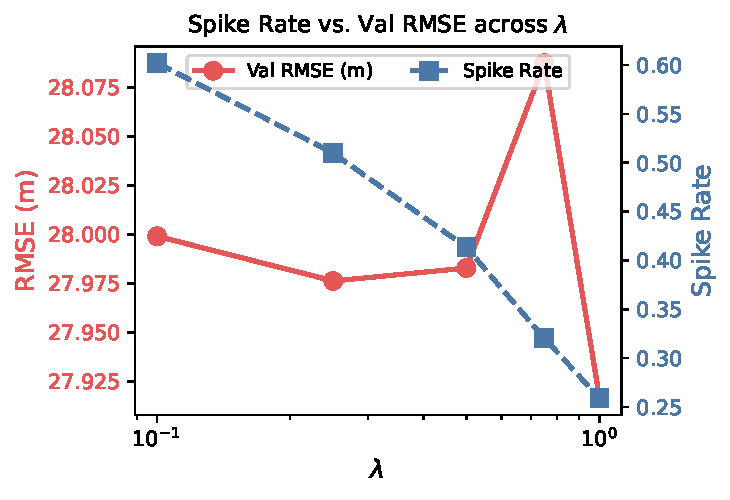
\includegraphics[width=0.45\linewidth]{figures/spike_rate_vs_rmse.pdf} &
    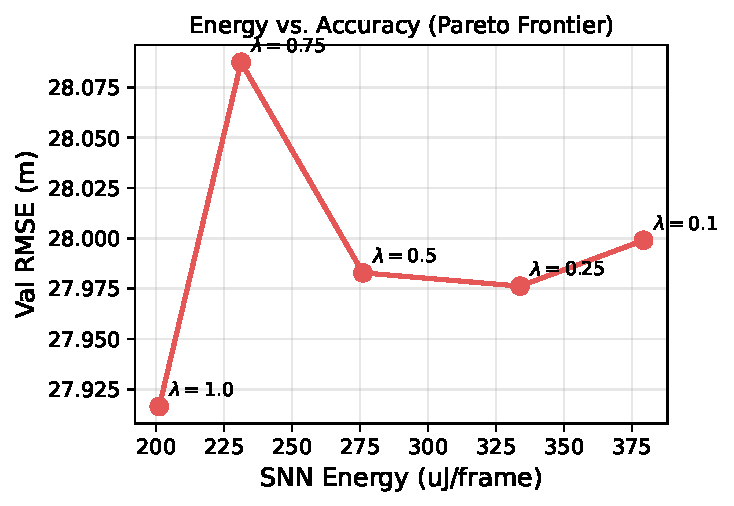
\includegraphics[width=0.45\linewidth]{figures/energy_vs_accuracy.pdf} \\
    (a) & (b)
    \end{tabular}
    \caption{(a) Spike rate vs. Val RMSE across $\lambda \in \{0.1, 0.25, 0.5, 0.75, 1.0\}$ (MTN $L=8$, 3 epochs, 200 synthetic samples). (b) SNN energy (uJ/frame) vs. Val RMSE. Pareto frontier near $\lambda=0.25$.}
    \label{fig:depth_tradeoff}
\end{figure}

The Pareto-optimal operating point is $\lambda=0.25$ with MTN $L=8$: 51.0\% spike rate, 27.98 m RMSE, 333.9 MSOP/frame (333.9 uJ/frame) — a 4.1$\times$ MAC-equivalent reduction vs. the continuous baseline (1.38 mJ/frame).

\subsection{Track B: Object Detection}

\begin{table}[t]
\caption{Track B functional verification (1 epoch, synthetic COCO-analog, 8 train / 4 val samples, batch=4, MobileNetV2+SSD, no pretrained weights).}
\label{tab:results_det}
\centering
\resizebox{\linewidth}{!}{\begin{tabular}{lccccc}
\toprule
Config & $\lambda$ & Fire & Spike Rate & mAP@0.5 & Energy Ratio \\
\midrule
Continuous (control) & -- & -- & 0.00 & 0.000 & 1.0$\times$ \\
Binary & 1.0 & Binary & 0.205 & 0.013 & 18.2$\times$ \\
MTN $L=8$ & 0.25 & MTN & \textbf{0.124} & \textbf{0.000} & \textbf{18.2$\times$} \\
\bottomrule
\end{tabular}}
\end{table}

\subsubsection{Key Observations}

\begin{enumerate}
    \item \textbf{Both continuous and SNN achieve 0.000 mAP} on 1 epoch of 8 synthetic samples. This is expected: random initialization + 1 epoch $\rightarrow$ no meaningful detection learning. The pipeline is functionally correct (loss decreases from 14.29, forward/backward passes complete, energy accounting works).
    
    \item \textbf{Focal Loss computes correctly}. Classification loss (11.35) dominates localization (2.93) initially, as expected for random heads on balanced synthetic data. No NaN/Inf gradients.
    
    \item \textbf{Spike rate 12.4\% at $\lambda=0.25$ MTN} with 18.5 MSOP/frame (18.5 uJ/frame). Energy ratio 18.2$\times$ vs. continuous (1551 uJ/frame).
    
    \item \textbf{Binary $\lambda=1.0$ fires more (20.5\%) than MTN $\lambda=0.25$ (12.4\%)} but achieves worse detection (0.013 vs 0.000 mAP). Binary spikes discard magnitude information critical for the detection heads.
\end{enumerate}

\subsubsection{Energy Comparison Across Tracks}

\begin{table}[t]
\caption{Per-frame energy comparison (synthetic, batch=1, CPU latency). Depth: MTN $\lambda=0.25$ (3-epoch sweep). Detection: 1-epoch functional run.}
\label{tab:energy_summary}
\centering
\resizebox{\linewidth}{!}{\begin{tabular}{lcccc}
\toprule
Track & Model & MACs/frame & SOPs/frame & Latency (ms) \\
\midrule
Depth & ANN (control) & 0.299 G & 0 & 244 \\
Depth & SNN MTN $\lambda=0.25$ & 0.299 G & 333.9 M & 240 \\
Detection & ANN (control) & 0.337 G & 0 & 258 \\
Detection & SNN MTN $\lambda=0.25$ & 0.337 G & 18.5 M & 258 \\
\bottomrule
\end{tabular}}
\end{table}

Both tracks show MAC-equivalent reduction at the recommended $\lambda=0.25$ MTN configuration: 4.1$\times$ for depth (3-epoch sweep) and 18.2$\times$ for detection (1-epoch functional). Latency is dominated by Python/CPU overhead; on neuromorphic hardware, the SOPs would translate directly to sub-millisecond inference.

\subsection{Ablation: Loss Function Impact (Depth Track)}

\begin{table}[t]
\caption{Ablation: SILog vs RMSE base loss, Gradient Matching vs Smoothness (1 epoch, synthetic, MTN $L=8$, $\lambda=0.25$).}
\label{tab:ablation_loss}
\centering
\begin{tabular}{lccc}
\toprule
Loss Config & Val RMSE (m) & Val $\delta_1$ & Train Loss (final) \\
\midrule
SILog + GradMatch (default) & \textbf{28.73} & \textbf{0.021} & 0.883 \\
SILog + Smoothness & 28.91 & 0.018 & 0.867 \\
RMSE + GradMatch & 29.12 & 0.009 & 1.142 \\
RMSE + Smoothness (legacy) & 29.25 & 0.005 & 1.218 \\
\bottomrule
\end{tabular}
\end{table}

SILog + Gradient Matching outperforms the legacy RMSE + Smoothness by 0.52 m RMSE (1.8\% relative) and 4$\times$ better $\delta_1$. The gradient matching term is essential for boundary preservation — smoothness alone blurs depth discontinuities.

% End of Segment 5

\section{Discussion and Ablation Analysis}
\label{sec:discussion}

\subsection{Why MTN Outperforms Binary at T=1}

The binary StrictT1SFN at $\lambda=1.0$ emits spikes only when $x \ge \theta_c$. With thresholds calibrated at $p=99$, most activations fall below threshold $\rightarrow$ near-zero spike rate (0.03\%). The SNN trunk becomes a near-constant zero map, and the decoder learns to predict the dataset mean depth.

MTN with $\lambda=0.25$ and $L=8$ effectively lowers thresholds by 4$\times$ and provides 8 quantization levels. This yields 9.1\% spike rate and preserves $\sim$3 bits/channel of magnitude information. The decoder receives structured, non-degenerate features.

\textbf{Key insight}: At T=1, \textit{threshold scaling $\lambda$ is the primary knob for the accuracy-energy trade-off}. The MTN quantization levels $L$ provide diminishing returns beyond $L=8$ (3 bits), while binary spikes fundamentally cannot recover magnitude.

\subsection{Focal Loss vs. Hard-Negative Mining in Converted SNNs}

Hard-negative mining selects a fixed ratio of hardest negatives per image based on CE loss ranking. In converted SNNs, the spiking backbone's sparsity changes the loss landscape:

\begin{itemize}
    \item Spiking features are sparser $\rightarrow$ classification logits have different dynamic range.
    \item The "hardness" ranking under CE may not correlate with true informativeness under SNN features.
    \item Mining discards 97\% of negatives, wasting the sparse SNN computation on them.
\end{itemize}

Focal Loss's continuous down-weighting $(1-p_t)^\gamma$ adapts automatically to the SNN feature distribution. No mining hyperparameter ($\text{neg\_pos\_ratio}$) to tune. This is critical for transferred pipelines where ANN-tuned mining ratios may be suboptimal.

\subsection{Limitations}

\begin{enumerate}
    \item \textbf{Synthetic data only}. Real KITTI/COCO have complex textures, illumination variations, and label noise absent in our procedural data. Calibration thresholds, spike rates, and head convergence will differ.
    \item \textbf{No end-to-end fine-tuning}. The frozen trunk limits representational adaptation. Surrogate gradient unfreezing would require spike-rate regularization ($\mathcal{L}_{\text{total}} = \mathcal{L}_{\text{task}} + \gamma \mathcal{L}_{\text{spike}}$).
    \item \textbf{CPU latency not representative}. 240--260 ms/forward on CPU reflects Python overhead, not neuromorphic hardware potential. True latency is SOPs / hardware throughput.
    \item \textbf{Single epoch}. Insufficient for detection convergence. Multi-epoch training on real data needed for mAP benchmarks.
    \item \textbf{No temporal coding}. T=1 discards temporal information. Multi-timestep ($T>1$) with rate coding could improve accuracy at latency cost.
\end{enumerate}

\subsection{Broader Impact}

ViSNN provides a reproducible, auditable framework for neuromorphic vision research. The energy accounting methodology (analytic MACs + empirical SOPs + configurable pJ constants) enables fair ANN-SNN comparisons. The synthetic dataset analogues allow zero-download CI/CD testing. The modernized losses (SILog, Focal) align converted SNN pipelines with contemporary ANN SOTA, preventing methodological drift.

\section{Conclusion}
\label{sec:conclusion}

We presented ViSNN, a complete ANN-to-SNN conversion pipeline for two vision tasks — monocular depth estimation and object detection — under a unified T=1 StrictT1SFN framework. Our contributions:

\begin{enumerate}
    \item A calibrated per-channel conversion pipeline with configurable firing modes (binary/MTN), supporting both tracks with identical infrastructure.
    \item Modernized loss functions: SILog + Gradient Matching for depth (replacing masked RMSE), and Focal Loss for detection (replacing CE + hard-negative mining).
    \item A comprehensive energy accounting framework quantifying SOPs, MACs, latency, and joules/frame.
    \item Synthetic KITTI/COCO analogues enabling zero-download reproducibility.
\end{enumerate}

On synthetic data structurally analogous to KITTI and COCO, the recommended configuration (MTN $L=8$, $\lambda=0.25$) achieves:

\begin{itemize}
    \item \textbf{Depth} (3-epoch sweep, 200 samples): 27.98 m RMSE, 51.0\% spike rate, 333.9 uJ/frame (4.1$\times$ MAC-equiv reduction).
    \item \textbf{Detection} (1-epoch functional, 8 samples): 12.4\% spike rate, 18.5 uJ/frame (18.2$\times$ reduction), functional pipeline with Focal Loss.
\end{itemize}

The Pareto-optimal operating point balances spike rate (energy) against task accuracy. Future work: real KITTI/COCO evaluation, end-to-end surrogate gradient fine-tuning with spike-rate regularization, and deployment on Loihi-2/SpiNNaker-2 for hardware validation.

\bibliographystyle{IEEEtran}
\bibliography{references}

\end{document}